\documentclass[tikz,border=3pt]{standalone}
\usepackage[utf8]{inputenc}
\usepackage[T1]{fontenc}
\usepackage{lmodern}
\renewcommand{\familydefault}{\sfdefault}
\usepackage{sansmath}\sansmath
\usepackage{pgfplots}\pgfplotsset{compat=1.18,/pgf/number format/use comma,/pgf/number format/1000 sep={.}}
\usetikzlibrary{arrows.meta,calc,positioning,decorations.pathmorphing,patterns}
% paleta del sitio
\definecolor{nar}{HTML}{E8680C}\definecolor{narc}{HTML}{FFB35C}\definecolor{hielo}{HTML}{FFF3E8}
\definecolor{tinta}{HTML}{1D1D1F}\definecolor{gris}{HTML}{6E6E73}\definecolor{lila}{HTML}{7C5CF0}
\definecolor{azul}{HTML}{2F6FD6}\definecolor{menta}{HTML}{17A673}\definecolor{coral}{HTML}{E8342A}
\begin{document}
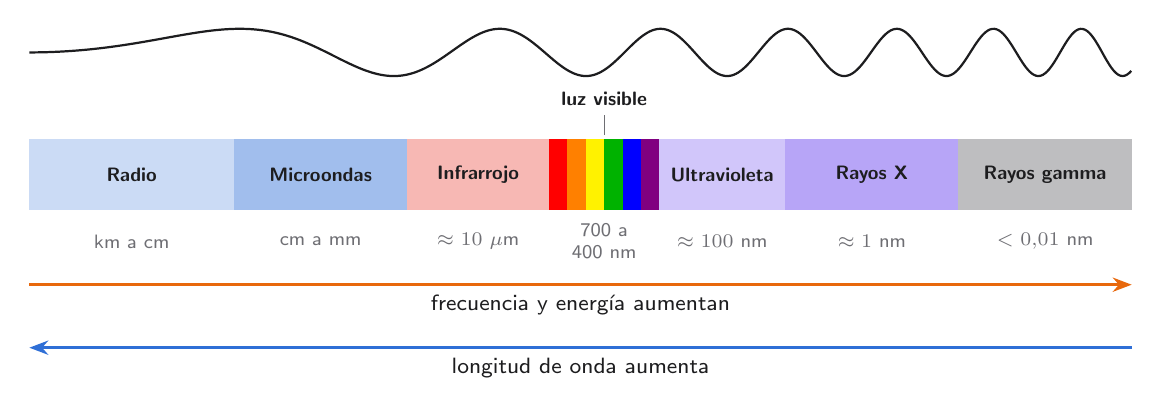
\begin{tikzpicture}[font=\footnotesize,>={Stealth[length=2.4mm]}]
\draw[thick,tinta,domain=0:14,samples=500,smooth] plot (\x,{2.0+0.3*sin(deg(0.22*\x*\x))});
\foreach \a/\b/\c/\t in {0/2.6/azul!25/Radio, 2.6/4.8/azul!45/Microondas, 4.8/6.6/coral!35/Infrarrojo, 8.0/9.6/lila!35/Ultravioleta, 9.6/11.8/lila!55/Rayos X, 11.8/14/gris!45/Rayos gamma}{
  \fill[\c] (\a,0) rectangle (\b,0.9); \node[font=\scriptsize\bfseries,text=tinta] at ({(\a+\b)/2},0.45) {\t};}
\foreach \i/\c in {0/red,1/orange,2/yellow,3/green!70!black,4/blue,5/violet} \fill[\c] ({6.6+0.2333*\i},0) rectangle ({6.6+0.2333*(\i+1)},0.9);
\draw[gris,thin] (7.3,0.95) -- (7.3,1.2) node[above,font=\scriptsize\bfseries,text=tinta] {luz visible};
\foreach \x/\t in {1.3/km a cm, 3.7/cm a mm, 5.7/{$\approx 10\ \mu$m}, 7.3/{700 a\\400 nm}, 8.8/{$\approx 100$ nm}, 10.7/{$\approx 1$ nm}, 12.9/{$< 0{,}01$ nm}}
  \node[font=\scriptsize,text=gris,align=center] at (\x,-0.4) {\t};
\draw[->,very thick,nar] (0,-0.95) -- (14,-0.95) node[midway,below,text=tinta] {frecuencia y energía aumentan};
\draw[->,very thick,azul] (14,-1.75) -- (0,-1.75) node[midway,below,text=tinta] {longitud de onda aumenta};
\end{tikzpicture}
\end{document}
